\documentclass{beamer}

\usetheme{default}
\usepackage[utf8]{inputenc}
\usepackage{tikz}
\usepackage{bm}
\usepackage{pgfplots}
\usepackage{graphicx}
\usepackage{gensymb}

\pgfplotsset{compat=1.4}
\usepgfplotslibrary{units}

\setbeamertemplate{footline}[frame number]
\setbeamertemplate{frametitle}[default][center]

\mode<presentation>{
	\usetheme{Dresden}
	%\setbeamercovered{transparent}
	\usecolortheme{seagull}
}

\setbeamertemplate{headline}{}

\definecolor{pemblue}{RGB}{1,123,165}
\setbeamercolor*{palette primary}{fg=black,bg=pemblue!80}
\setbeamercolor*{palette secondary}{fg=black,bg=pemblue!80!gray!80}
\setbeamercolor*{palette tertiary}{fg=black,bg=pemblue!100}
\setbeamercolor*{palette quaternary}{fg=black,bg=pemblue!110}

\usebackgroundtemplate
{%
	\begin{picture}(210,40)(-5,2)
	
\includegraphics[width=0.07\paperwidth,keepaspectratio]{imgs/pem-logo-short.png}
	\end{picture}%
}

\title{Estimativa
	de condutâncias térmicas de contato em interfaces irregulares usando a
	técnica da Transformada Integral Clássica e o método dos funcionais de reciprocidade}
\author{Guilherme Camelo de Freitas}
\date{29 de Junho de 2019}

\institute
{
	Universidade Federal do Rio de Janeiro\\
	UFRJ/COPPE/PEM
}


% Let's get started
\begin{document}
	
	{
		\usebackgroundtemplate{
			\begin{picture}(210,55)(-5,0)
			
\includegraphics[height=0.14\paperwidth,keepaspectratio]{imgs/pem-logo.png}
			\end{picture}%
			\begin{picture}(210,55)(-28,2)
			
\includegraphics[height=0.14\paperwidth,keepaspectratio]{imgs/coppe-logo.pdf}
			\end{picture}
		}
		\begin{frame}
			\bigskip\bigskip\bigskip\bigskip
			\titlepage
		\end{frame}
	}
	
	\begin{frame}{Agenda}
		\tableofcontents
	\end{frame}

\section{Introdução}

\begin{frame}
	\frametitle{Introdução}
	\begin{figure}[h!b]
		\begin{center}
			\begin{tikzpicture}
			\node at (0, 0)
			{
				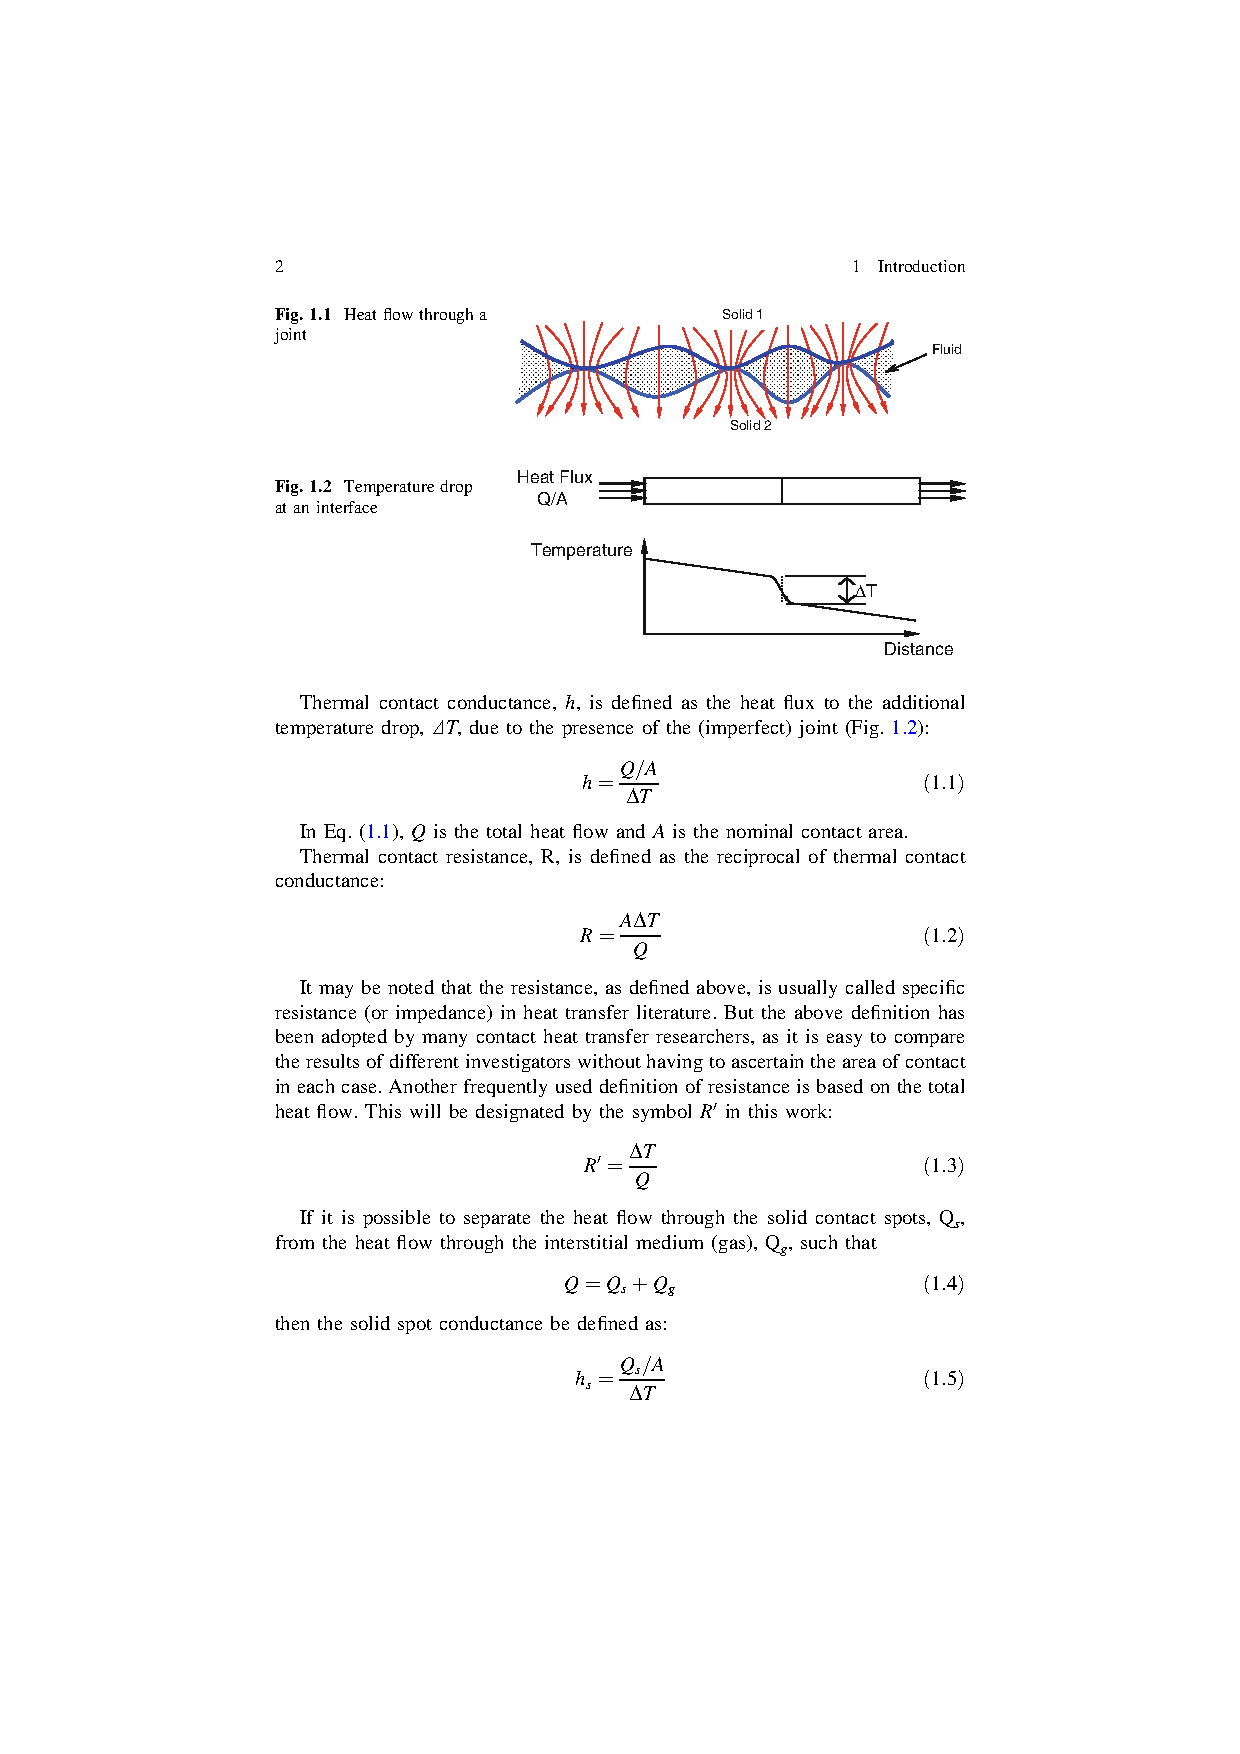
\includegraphics[trim=250 642 150 154, clip=true]{imgs/img1.pdf}
			};
			
			\node[scale=0.8] at (0, 0.9) {Sólido 1};
			\node[scale=0.8] at (0, -1.1) {Sólido 2};
			\node[scale=0.8] at (4, 0.3) {Fluido};
			\end{tikzpicture}
		\end{center}
	\end{figure}
\end{frame}

\begin{frame}
	\frametitle{Introdução}
	\framesubtitle{Definição de condutância térmica de contato}
	\begin{equation}
	h_c = \frac{q_c}{\Delta T_c}
	\end{equation}
\end{frame}

\section{Problema físico}

\begin{frame}
	\frametitle{Problema físico}
	\framesubtitle{Arranjo físico}
	\begin{figure}[h!b]
		\begin{center}
			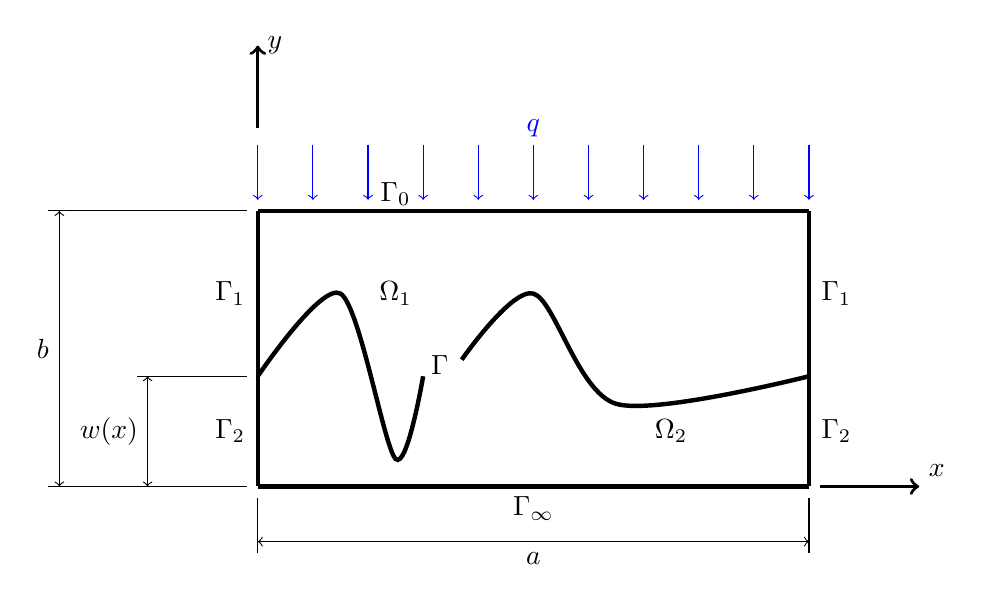
\begin{tikzpicture}[scale=0.7]
			
			\draw [ultra thick] (0, 0) -- (10, 0);
			%\draw [ultra thick] (0, 2) -- (7, 2);
			%\draw [ultra thick] (8, 2) -- (10, 2);
			\draw [ultra thick] plot [smooth] coordinates {(0, 2) (1.5, 3.5) (2.5, 0.5) (3, 2)};
			\draw [ultra thick] plot [smooth] coordinates {(3.7, 2.3) (5, 3.5) (6.5, 1.5) (10, 2)};
			\draw [ultra thick] (0, 5) -- (10, 5);
			\draw [ultra thick] (0, 0) -- (0, 5);
			\draw [ultra thick] (10, 0) -- (10, 5);
			
			\draw (2.5, 3.5) node {$\Omega_1$};
			\draw (7.5, 1) node {$\Omega_2$};	
			\draw (3.3, 2.2) node {$\Gamma$};
			\draw (-0.5, 3.5) node {$\Gamma_1$};
			\draw (-0.5, 1) node {$\Gamma_2$};
			\draw (10.5, 3.5) node {$\Gamma_1$};
			\draw (10.5, 1) node {$\Gamma_2$};
			\draw (5, -0.4) node {$\Gamma_\infty$};
			\draw (2.5, 5.3) node {$\Gamma_0$};
			\draw [blue](5, 6.5) node {$q$};
			\draw (5, -1.3) node {$a$};
			\draw (-3.9, 2.5) node {$b$};
			\draw (-2.7, 1) node {$w(x)$};
			
			\node [above right] at (12, 0) {$x$};
			\node [right] at (0, 8) {$y$};
			
			\draw [->, blue] (0, 6.2) -- (0, 5.2);
			\draw [->, blue] (1, 6.2) -- (1, 5.2);
			\draw [->, blue] (2, 6.2) -- (2, 5.2);
			\draw [->, blue] (3, 6.2) -- (3, 5.2);
			\draw [->, blue] (4, 6.2) -- (4, 5.2);
			\draw [->, blue] (5, 6.2) -- (5, 5.2);
			\draw [->, blue] (6, 6.2) -- (6, 5.2);
			\draw [->, blue] (7, 6.2) -- (7, 5.2);
			\draw [->, blue] (8, 6.2) -- (8, 5.2);
			\draw [->, blue] (9, 6.2) -- (9, 5.2);
			\draw [->, blue] (10, 6.2) -- (10, 5.2);
			
			\draw [->, very thick] (10.2,0) -- (12,0);
			\draw [->, very thick] (0, 6.5) -- (0,8);
			
			\draw [-] (0, -0.2) -- (0, -1.2);
			\draw [-] (10, -0.2) -- (10, -1.2);
			\draw [<->] (0, -1) -- (10, -1);
			
			\draw [-] (-0.2, 0) -- (-3.8, 0);
			\draw [-] (-0.2, 5) -- (-3.8, 5);
			\draw [-] (-0.2, 2) -- (-2.2, 2);
			\draw [<->] (-3.6, 0) -- (-3.6, 5);
			\draw [<->] (-2.0, 0) -- (-2.0, 2);
			
			\end{tikzpicture}
		\end{center}
	\end{figure}
\end{frame}

\begin{frame}
	\frametitle{Problema físico}
	\framesubtitle{Formulação}
	\begin{subequations}
		\begin{alignat}{2}
		& \nabla^2 F_{1,j} = 0 \quad\quad\quad\quad\quad && \text{ in } \Omega_1 \label{funcao_F_harm_T1} \\
		& F_{1,j} = \psi_j && \text{ on } \Gamma_0  \label{funcao_F_cc_T1_2} \\
		& \frac{\partial F_{1,j}}{\partial \mathbf{n}_1} = 0 && \text{ on }  \Gamma_1 \label{funcao_F_cc_T1_1} \\ 
		& F_{1,j} = F_{2, j} \quad\quad\quad\quad\quad\quad\quad\quad && \text{ on }  \Gamma \label{funcao_F_cc_grad_T1} \\
		& \nabla^2 F_{2,j} = 0 && \text{ in }  \Omega_2 \label{funcao_F_harm_T2} \\
		& \frac{\partial F_{2,j}}{\partial \mathbf{n}_2} = 0 && \text{ on }  \Gamma_2 \label{funcao_F_cc_T1_3} \\
		& F_{2,j} = 0 && \text{ on }  \Gamma_\infty \label{funcao_F_cc_T1_4} \\
		& k_2\frac{\partial F_{2, j}}{\partial\mathbf{n}_2} = - k_1\frac{\partial F_{1,j}}{\partial\mathbf{n}_1} && \text{ on }  \Gamma \label{funcao_F_cc_T1_5}
		\end{alignat}
	\end{subequations}
\end{frame}

\begin{frame}
	Definição do funcional de reciprocidade (citar)
	\begin{align}
	\Re(F) = \int_{\Gamma_0}\left[\left(\frac{-q}{k_1}\right)F - Y\frac{\partial F}{\partial\mathbf{n_1}}\right]d\Gamma_0
	\label{def_funcional_reciprocidade}
	\end{align}
\end{frame}

\begin{frame}
	Identidades
	
	\begin{align}
	k_1\int_{\Gamma_0}\left[\left(\frac{-q}{k_1}\right)\right. & \left.F_1 - Y\frac{\partial F_1}{\partial\mathbf{n_1}}\right]d\Gamma_0
	=\int_\Gamma k_1 \frac{\partial F_1}{\partial\mathbf{n_1}}\left(T_1 - T_2\right)d\Gamma
	\label{identidade_T} \\ \nonumber \\
	k_1\int_{\Gamma_0}\left[\left(\frac{-q}{k_1}\right)\right. & \left.G_1 -  Y\frac{\partial G_1}{\partial\mathbf{n_1}}\right]d\Gamma_0
	= \int_\Gamma -k_1 G_1 \frac{\partial T_1}{\partial\mathbf{n_1}}d\Gamma
	\label{identidade_q}
	\end{align}
	
\end{frame}

\begin{frame}
	\begin{table}[H]
		\centering
		\caption{Parâmetros usados nos problemas-teste}
		\begin{tabular}{|l|l|}
			\hline
			\textbf{Parâmeytro} & \textbf{Valor}  \\ \hline
			$a$       & 0.04 m   \\ \hline
			$b$       & 0.02 m     \\ \hline
			$k_1$     & 54 W/(m \celsius)  \\ \hline
			$k_2$     & 14 W/(m \celsius) \\ \hline
			$q$       & -100,000 W/$\text{m}^2$ \\ \hline
			$h_{max}$       & 1000 W/($\text{m}^2$ \celsius) \\ \hline
		\end{tabular}		
		\label{tabela_params}
	\end{table}
\end{frame}


\begin{frame}
	\begin{table}[H]
		\centering
		\caption{Geometrias de interface de contato}
		\begin{tabular}{|l|l|}
			\hline 
			\textbf{Geometry} & \textbf{Expression for} $w(x)$    \\ \hline
			1       & $\frac{b}{2}$   \\ \hline
			2       & $\begin{array}{ll}
			\frac{19bx^2}{8a^2}-\frac{7bx}{24a}+\frac{b}{2}, &  0 \le x < \frac{a}{3} \\
			-\frac{25bx^2}{8a^2}+\frac{27bx}{8a}-\frac{b}{9}, &  \frac{a}{3} \le x < \frac{2a}{3} \\ 
			\frac{bx^2}{8a^2}-\frac{23bx}{24a}+\frac{4b}{3}, &  \frac{2a}{3} \le x \le a
			\end{array}$     \\ \hline
			3       & $ \frac{b}{2} + \frac{1}{20} \cos\frac{4 \pi  x}{a}$ \\ \hline
		\end{tabular}			
		\label{tabela_interfaces}
	\end{table}
\end{frame}

\begin{frame}
	\begin{figure}[H]
		\begin{minipage}[t][5cm][c]{\textwidth}
			\centering
			\begin{tikzpicture}
			\begin{axis}[
			anchor=east,  
			ticks=none,
			width=8cm,
			height=4cm,
			%ylabel=Iterações Lineares,
			xmin = 0,
			xmax = 0.04,
			ymin = 0,
			ymax = 0.02]
			\pgfplotstableread{../data/interface_01.dat} 
			\teff
			\addplot[color=blue,mark=none,smooth] table from \teff;
			\end{axis}
			\end{tikzpicture}
			\caption*{(a) Geometria 1}
		\end{minipage}
		%	\begin{minipage}[t][5cm][t]{0,5\textwidth}
		%		\begin{tikzpicture}
		%		\begin{axis}[
		%		anchor=east,  
		%		ticks=none,
		%		width=8cm,
		%		height=4cm,
		%		%ylabel=Iterações Lineares,
		%		xmin = 0,
		%		xmax = 0.04,
		%		ymin = 0,
		%		ymax = 0.02]
		%		\pgfplotstableread{../data/interface_05.dat} 
		%		\teff
		%		\addplot[color=blue,mark=none,smooth] table from \teff;
		%		\end{axis}
		%		\end{tikzpicture}
		%		\caption*{(b) Geometria 2}
		%	\end{minipage}
		%	\begin{minipage}[t][5cm][t]{0,5\textwidth}
		%		\begin{tikzpicture}
		%		\begin{axis}[
		%		anchor=east,  
		%		ticks=none,
		%		width=8cm,
		%		height=4cm,
		%		%ylabel=Iterações Lineares,
		%		xmin = 0,
		%		xmax = 0.04,
		%		ymin = 0,
		%		ymax = 0.02]
		%		\pgfplotstableread{../data/interface_06.dat} 
		%		\teff
		%		\addplot[color=blue,mark=none,smooth] table from \teff;
		%		\end{axis}
		%		\end{tikzpicture}
		%		\caption*{(c) Geometria 3}
		%	\end{minipage}
		\begin{minipage}[t][5cm][c]{\textwidth}
			\centering
			\begin{tikzpicture}
			\begin{axis}[
			anchor=east,  
			ticks=none,
			width=8cm,
			height=4cm,
			%ylabel=Iterações Lineares,
			xmin = 0,
			xmax = 0.04,
			ymin = 0,
			ymax = 0.02]
			\pgfplotstableread{../data/interface_02.dat} 
			\teff
			\addplot[color=blue,mark=none,smooth] table from \teff;
			\end{axis}
			\end{tikzpicture}
			\caption*{(d) Geometria 2}
		\end{minipage}
		%	\begin{minipage}[t][5cm][t]{0,5\textwidth}
		%		\begin{tikzpicture}
		%		\begin{axis}[
		%		anchor=east,  
		%		ticks=none,
		%		width=8cm,
		%		height=4cm,
		%		%ylabel=Iterações Lineares,
		%		xmin = 0,
		%		xmax = 0.04,
		%		ymin = 0,
		%		ymax = 0.02]
		%		\pgfplotstableread{../data/interface_08.dat} 
		%		\teff
		%		\addplot[color=blue,mark=none,smooth] table from \teff;
		%		\end{axis}
		%		\end{tikzpicture}
		%		\caption*{(e) Geometria 5}
		%	\end{minipage}
		\begin{minipage}[t][5cm][c]{\textwidth}
			\centering
			\begin{tikzpicture}
			\begin{axis}[
			anchor=east,  
			ticks=none,
			width=8cm,
			height=4cm,
			%ylabel=Iterações Lineares,
			xmin = 0,
			xmax = 0.04,
			ymin = 0,
			ymax = 0.02]
			\pgfplotstableread{../data/interface_03.dat} 
			\teff
			\addplot[color=blue,mark=none,smooth] table from \teff;
			\end{axis}
			\end{tikzpicture}
			\caption*{(f) Geometria 3}
		\end{minipage}	
		\caption{Diferentes geometrias para a interface $\Gamma$}
		\label{figura_interfaces}
	\end{figure}
\end{frame}
	
	
	
\end{document}